\documentclass[a4paper,11.5pt, table]{article}

%%%%%% Basic packages begin %%%%%%
\usepackage[
	textwidth  = 160mm, 
	textheight = 230mm, 
	top        = 25mm, 
	bottom     = 30mm
]{geometry}
\usepackage[normalem]{ulem}
\usepackage[utf8]{inputenc}
\usepackage[T1]{fontenc}
\PassOptionsToPackage{defaults=hu-min}{magyar.ldf}
\usepackage[magyar]{babel}

%%%%%%% Basic packages end %%%%%%%

%%%%%% Packages required for this document begin %%%%%%
\usepackage{
	amsmath,   % Math mode
	amsthm,    % "note" environment
	amsfonts,  % "\mathbb{}" command
	paralist,  % "compactitem" and "compactenum" environment
	multirow,  % "\multirow{}{}" command
	float,     % "H" float specifier
	tikz,      % Basepackage for nearly all figures
	listings,  % Used for code snippets
	etaremune, % Reverse compactenum
%	graphicx   % For including images
	enumitem   %for alphabetical enumeration
}
\usepackage[unicode]{hyperref} % Clickable links
%%%%%%% Packages required for this document end %%%%%%%

%%%%%% TikZ options start %%%%%%
\usetikzlibrary{
	positioning, % Contains positioning utilities, such as "below = of" 
	calc,        % Adding coordinates
	math         % Needed for global variables
}

\tikzstyle{NodeBase} = [
	rectangle,
	text centered,
	draw = black
]

\definecolor{DefaultObjectColor}{gray}{0.9} % This is the default color of object in the TikZ pictures

\tikzstyle{arrow} = [
	thick,
	->,
	>=stealth
]
%%%%%%% TikZ options end %%%%%%%

%%%%%% lstlistings envvironment options start %%%%%%

\lstdefinestyle{customc}{ % C/C++ code snippet style
	belowcaptionskip = 1\baselineskip,
	breaklines       = true,
	frame            = L, % Double line on the left
	language         = C++,
	showstringspaces = false,
	basicstyle       = \ttfamily,
	keywordstyle     = \bfseries\color{green!40!black},
	stringstyle      = \color{orange},
	emphstyle        = \color{blue}, % Defined below
	tabsize          = 4,
	columns          = fullflexible,
}

\lstset{
	escapechar = @,
	style      = customc, % Default code snippet style
	%NOTE In order to use special characters in code snippets, one has to manually define them.
	literate   = {á}{{\'a}}1 {é}{{\'e}}1 {í}{{\'i}}1 {ó}{{\'o}}1 {ú}{{\'u}}1	{Á}{{\'A}}1 {É}{{\'E}}1 {Í}{{\'I}}1 {Ó}{{\'O}}1 {Ú}{{\'U}}1	{ö}{{\"o}}1 {ü}{{\"u}}1 {Ö}{{\"O}}1 {Ü}{{\"U}}1
	{ű}{{\H{u}}}1 {Ű}{{\H{U}}}1 {ő}{{\H{o}}}1 {Ő}{{\H{O}}}1
	{€}{{\euro}}1 {£}{{\pounds}}1 {~}{$\sim$}{1}	
}

%%%%%%% lstlistings envvironment options end %%%%%%%

%%%%%%%% Compilation error fix begin %%%%%%%%
\makeatletter
\expandafter\let\csname active@char\string?\endcsname\relax
\expandafter\let\csname active@char\string!\endcsname\relax
\expandafter\let\csname active@char\string:\endcsname\relax

\initiate@active@char{?}
\initiate@active@char{!}
\initiate@active@char{:}
\makeatletter
%%%%%%%%% Compilation error fix end %%%%%%%%%

\setlength{\parindent}{0mm}
\setlength{\parskip}{1em}
\setcounter{section}{0}

\begin{document}
	\begin{center}
		{\Huge Adatbázisok II}
		\smallskip
		
		{\Large VI. Ellenőrzőkérdések}
	\end{center}
189. Milyen problémát kell megoldania a konkurrencia-vezérlésnek? (4 pont)
	\begin{compactitem}
		\item A tranzakciók közötti egymásra hatás az adatbázis-állapot inkonzisztenssé válását okozhatja, még akkor is, amikor a tranzakciók külön-külön megőrzik a konzisztenciát, és rendszerhiba sem történt. 
		\item \textit{MJ.: Akkor fordulhat elő ilyen, ha két, egyszerre futó tranzakció ugyan azt az adatrészt módosítja.}
	\end{compactitem}

190. Mit hívunk ütemezőnek? (2 pont)
	\begin{compactitem}
		\item Az adatbázis-kezelő azon részét hívjuk ütemezőnek (scheduler), amely a tranzakciós lépések szabályozásának feladatát végzi.
	\end{compactitem}

191. Mit hívunk ütemezésnek? (2 pont)
	\begin{compactitem}
		\item Az ütemezés \textit{(schedule)} egy vagy több tranzakció által végrehajtott lényeges műveletek időrendben vett sorozata, amelyben az egy tranzakcióhoz tartozó műveletek sorrendje megegyezik a tranzakcióban megadott sorrenddel. 
	\end{compactitem}

192. Milyen 2 módon biztosítja az ütemező a sorbarendezhetőséget? (2 pont)
	\begin{compactitem}
		\item Várakoztat, abortot rendel el, hogy a sorbarendezhetőséget biztosítsa.
	\end{compactitem}

193. Mit hívunk konfliktuspárnak? (2 pont)
	\begin{compactitem}
		\item A konfliktus \textit{(conflict)} vagy konfliktuspár olyan egymást követő műveletpár az ütemezésben, amelynek ha a sorrendjét felcseréljük, akkor legalább az egyik tranzakció viselkedése megváltozhat.
	\end{compactitem}

194. Milyen 3 esetben nem cserélhetjük fel a műveletek sorrendjét, mert inkonzisztenciát okozhatna? (3 pont)
\begin{compactitem}
	\item Legyen T$_{i}$ és T$_{j}$ két különböző tranzakció (i $\not=$ j).
	\begin{enumerate}[label= \alph*)]
		\item r$_{i}$(X); w$_{i}$(Y) konfliktus,
		\begin{compactitem}
			\item M
			ivel egyetlen tranzakción belül a műveletek sorrendje rögzített, és az adatbázis-kezelő ezt a sorrendet nem rendezheti át.
		\end{compactitem}
		
		\item w$_{i}$(X); w$_{j}$(X) konfliktus, 
		\begin{compactitem}
			\item Mivel mind a kettőt ugyan azt az adatot módosítja. (Ha felcserélnénk őket, más lehet az eredmény.)
		\end{compactitem}
		
		\item r$ _{i} $(X); w$ _{j} $(X) és w$ _{i} $(X); r$ _{j} $(X) is konfliktus. 
		\begin{compactitem}
			\item Ha megcserélnénk a sorrendet, egyrészt az írások miatt más lenne az olvasott adat, másrészt a felcserélt írások sorrendje miatt X értékének a 4 művelet utáni változata is megváltozhat. (És ez a csere azt is jelentené, hogy tranzakción belüli sorrendet cserélünk fel.)
		\end{compactitem}
	\end{enumerate}
\end{compactitem}

195. Mikor konfliktus-ekvivalens 2 ütemezés? (2 pont)
	\begin{compactitem}
		\item Azt mondjuk, hogy két ütemezés konfliktusekvivalens \textit{(conflict-equivalent)}, ha szomszédos műveletek nem konfliktusos cseréinek sorozatával az egyiket átalakíthatjuk a másikká. 
	\end{compactitem}

196. Mikor konfliktus-sorbarendezhető egy ütemezés? (2 pont)
	\begin{compactitem}
		\item Azt mondjuk, hogy egy ütemezés konfliktus-sorbarendezhető \textit{(conflict-serializable schedule)}, ha konfliktusekvivalens valamely soros ütemezéssel. 
		\item \textit{MJ.: Azaz nem konfliktusos cserékkel átvihető az egyik a másikba.}
	\end{compactitem}

197. Mi a konfliktus-sorbarendezhetőség elve? (3 pont)
	\begin{compactitem}
		\item ELV: nem konfliktusos cserékkel az ütemezést megpróbáljuk soros ütemezéssé átalakítani. Ha ezt meg tudjuk tenni, akkor az eredeti ütemezés sorbarendezhető volt, ugyanis az adatbázis állapotára való hatása változatlan marad minden nem konfliktusos cserével.
	\end{compactitem}

198. Mi a kapcsolat a sorbarendezhetőség és a konfliktus-sorbarendezhetőség között? (2 pont)
	\begin{compactitem}
		\item Azt mondjuk, hogy egy ütemezés konfliktus-sorbarendezhető \textit{(conflict-serializable schedule)}, ha konfliktusekvivalens valamely soros ütemezéssel. 
		\begin{compactitem}
			\item Azaz nem konfliktusos cserék által valamely soros ütemezést kaphatjuk.
		\end{compactitem}
		
		\item A konfliktus-sorbarendezhetőség elégséges feltétel a sorbarendezhetőségre, vagyis egy konfliktus-sorbarendezhető ütemezés sorbarendezhető ütemezés is egyben. 
	\end{compactitem}

199. Az r$ _{1} $(A); w$ _{1} $(A); r$ _{2} $(A); w$ _{2} $(A); r$ _{1} $(B); w$ _{1} $(B); r$ _{2} $(B); w$ _{2} $(B); ütemezést alakítsuk soros ütemezéssé (5 pont)
	\begin{compactitem}
		\item Azt állítjuk, hogy ez az ütemezés konfliktus-sorbarendezhető. A következő cserékkel ez az ütemezés átalakítható a (T$ _{1} $, T$ _{2} $) soros ütemezéssé, ahol az összes T$ _{1} $-beli művelet megelőzi az összes T$ _{2} $-beli műveletet:
	\end{compactitem}
\begin{figure}[h]
	\centering
	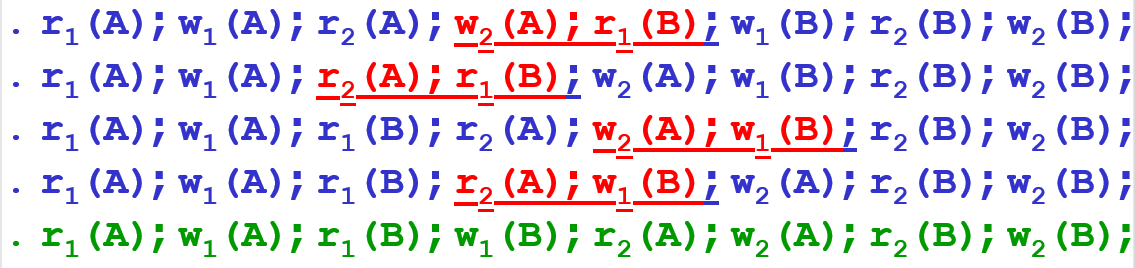
\includegraphics[height=3cm]{01.png}
\end{figure}

200. Adjunk példát sorbarendezhető, de nem konfliktus-sorbarendezhető ütemezésre (4 pont)
	\begin{compactitem}
		\item S$ _{2} $: w$ _{1} $(Y); w$ _{2} $(Y); w$ _{2} $(X); w$ _{1} $(X); w$ _{3} $(X);
	\end{compactitem}

201. Mi a konfliktus-sorbarendezhetőség tesztelésének alapötlete? (2 pont)
	\begin{compactitem}
		\item Alapötlet: ha valahol konfliktusban álló műveletek szerepelnek S-ben, akkor az ezeket a műveleteket végrehajtó tranzakcióknak ugyanabban a sorrendben kell előfordulniuk a konfliktus-ekvivalens soros ütemezésekben, mint ahogyan az S-ben voltak.
	\end{compactitem}

202. Mikor mondjuk, hogy egy S ütemezés alapján T$ _{1} $ megelőzi T$ _{2} $-t? (5 pont)
	\begin{compactitem}
		\item Adott a T$ _{1} $ és T$ _{2} $, esetleg további tranzakcióknak egy S ütemezése. Azt mondjuk, hogy T$ _{1} $ megelőzi T$ _{2} $‑t, ha van a T$ _{1} $-ben olyan A$ _{1} $ művelet és a T$ _{2} $-ben olyan A$ _{2} $ művelet, hogy
		\begin{enumerate}
			\item A$ _{1} $ megelőzi A$ _{2} $-t S-ben,
			\item A$ _{1} $ és A$ _{2} $ ugyanarra az adatbáziselemre vonatkoznak, és
			\item A$ _{1} $ és A$ _{2} $ közül legalább az egyik írás művelet.
		\end{enumerate}
		\item MJ.:
		\begin{compactitem}
			\item Másképpen fogalmazva: A$ _{1} $ és A$ _{2} $ konfliktuspárt alkotna, ha szomszédos műveletek lennének. Jelölése: T$ _{1} $ <$ _{S} $ T$ _{2} $. 
			\item Látható, hogy ezek pontosan azok a feltételek, amikor nem lehet felcserélni A$ _{1} $ és A$ _{2} $ sorrendjét. Tehát A$ _{1} $ az A$ _{2} $ előtt szerepel bármely S-sel konfliktusekvivalens ütemezésben. Ebből az következik, hogy ha ezek közül az ütemezések közül az egyik soros ütemezés, akkor abban T$ _{1} $-nek meg kell előznie T$ _{2} $‑t.
		\end{compactitem}
	\end{compactitem}

203. Adjuk meg egy S ütemezéshez tartozó megelőzési gráf definícióját! (5 pont)
	\begin{compactitem}
		\item Az utóbbi kérdésnél leírt megelőzéseket a megelőzési gráfban \textit{(precedence graph)} összegezhetjük. A megelőzési gráf csúcsai az S ütemezés tranzakciói. Ha a tranzakciókat T$ _{i} $-vel jelöljük, akkor a T$ _{i} $-nek megfelelő csúcsot az i egész jelöli. Az i csúcsból a j csúcsba akkor vezet irányított él, ha T$ _{i} $ <S T$ _{j} $.
	\end{compactitem}

204. Milyen kapcsolat van a konfliktus-ekvivalencia és a megelőzési gráfok között? (4 pont)
	\begin{compactitem}
		\item Lemma: S$ _{1} $, S$ _{2} $ konfliktusekvivalens $ \implies $ gráf(S$ _{1} $) = gráf(S$ _{2} $)
		\item Megjegyzés: gráf(S$ _{1} $) = gráf(S$ _{2} $) $ \not\Rightarrow $ S$ _{1} $, S$ _{2} $ konfliktusekvivalens
	\end{compactitem}

205. Adjunk példát arra, hogy két ütemezés megelőzési gráfja megegyezik, de nem konfliktus-ekvivalensek!(4 pont)
	\begin{compactitem}
		\item Ellenpélda:
		\begin{compactitem}
			\item S$ _{1} $=w$ _{1} $(A) r$ _{2} $(A) w$ _{2} $(B) r$ _{1} $(B)
			\item S$ _{2} $=r$ _{2} $(A) w$ _{1} $(A) r$ _{1} $(B) w$ _{2} $(B)
		\end{compactitem}
			\begin{figure}[h]
				\centering
				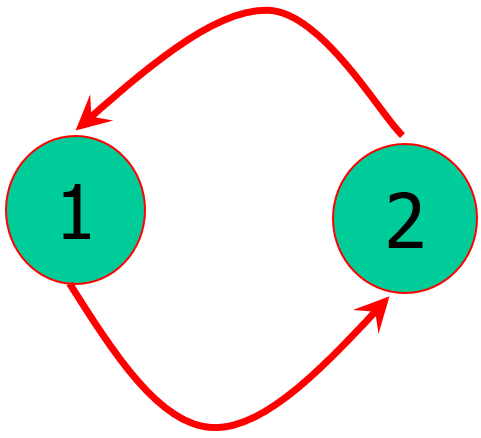
\includegraphics[height=3cm]{02.png}
			\end{figure}
	\end{compactitem}


206. Mit hívunk egy irányított, körmentes gráf esetében a csúcsok topologikus sorrendjének? (4 pont)
	\begin{compactitem}
		\item Egy körmentes gráf csúcsainak topologikus sorrendje a csúcsok bármely olyan rendezése, amelyben minden \textit{a $ \rightarrow $ b} élre az \textit{a} csúcs megelőzi a \textit{b} csúcsot a topologikus rendezésben.
	\end{compactitem}

207. Hogyan lehet tesztelni a megelőzési gráf alapján egy ütemezés konfliktus-sorbarendezhetőségét? (4 pont)
	\begin{compactitem}
		\item Ha az S megelőzési gráf tartalmaz irányított kört, akkor S nem konfliktus-sorbarendezhető, ha nem tartalmaz irányított kört, akkor S konfliktus-sorbarendezhető, és a csúcsok bármelyik topologikus sorrendje megadja a konfliktusekvivalens soros sorrendet.
	\end{compactitem}

208. Mi jellemző a passzív ütemezésre? (4 pont)
	\begin{compactitem}
		\item \textit{MJ.: A passzív ütemezés az ütemező egy eszköze a sorbarendezhetőség elérésére.}
		\item Passzív módszer: 
		\begin{enumerate}
			\item hagyjuk a rendszert működni, 
			\item az ütemezésnek megfelelő gráfot tároljuk, 
			\item egy idő után megnézzük, hogy van-e benne kör, 
			\item és ha nincs, akkor szerencsénk volt, jó volt az ütemezés.
		\end{enumerate}
	\end{compactitem}

209. Mi jellemző az aktív ütemezésre és milyen 3 módszert lehet erre használni? (5 pont)
	\begin{compactitem}
		\item \textit{MJ.: Az aktív ütemezés az ütemező egy eszköze a sorbarendezhetőség elérésére.}
		\item Aktív módszer: az ütemező beavatkozik, és megakadályozza, hogy kör alakuljon ki. 
		\item Az ütemezőnek több lehetősége is van arra, hogy kikényszerítse a sorbarendezhető ütemezéseket:
		\begin{compactitem}
			\item zárak (ezen belül is még: protokoll elemek, pl. 2PL)
			\item időbélyegek (time stamp)
			\item érvényesítés
		\end{compactitem}
		\item \textit{Fő elv: inkább legyen szigorúbb és ne hagyjon lefutni egy olyan ütemezést, ami sorbarendezhető, mint hogy fusson egy olyan, ami nem az.}
	\end{compactitem}

\section{Zárak használata}

210. Mit hívunk a tranzakciók konzisztenciájának zárolási ütemező esetén? (2 pont)
	\begin{compactitem}
		\item \textit{MJ:: A zárolási ütemező a konfliktus-sorbarendezhetőséget követeli meg, (ez erősebb követelmény, mint a sorbarendezhetőség).}
		\item Tranzakciók konzisztenciája (consistency of transactions):
		\begin{compactitem}
			\item A tranzakció csak akkor olvashat vagy írhat egy elemet, ha már korábban zárolta azt, és még nem oldotta fel a zárat.
			\item Ha egy tranzakció zárol egy elemet, akkor később azt fel kell szabadítania.
		\end{compactitem}
	\end{compactitem}
	
211. Mit hívunk a zárolási ütemező jogszerűségének? (1 pont)
	\begin{compactitem}
		\item Az ütemezések jogszerűsége\textit{ (legality of schedules)}: 
		Nem zárolhatja két tranzakció ugyanazt az elemet, csak úgy, ha az egyik előbb már feloldotta a zárat.
	\end{compactitem}

212. Adjunk példát konzisztens tranzakciók jogszerű ütemezésére, ami mégsem sorbarendezhető! (6 pont)
	\begin{compactitem}
		\item Ez az ütemezés jogszerű, de nem sorba rendezhető. 
		\begin{figure}[h]
			\centering
			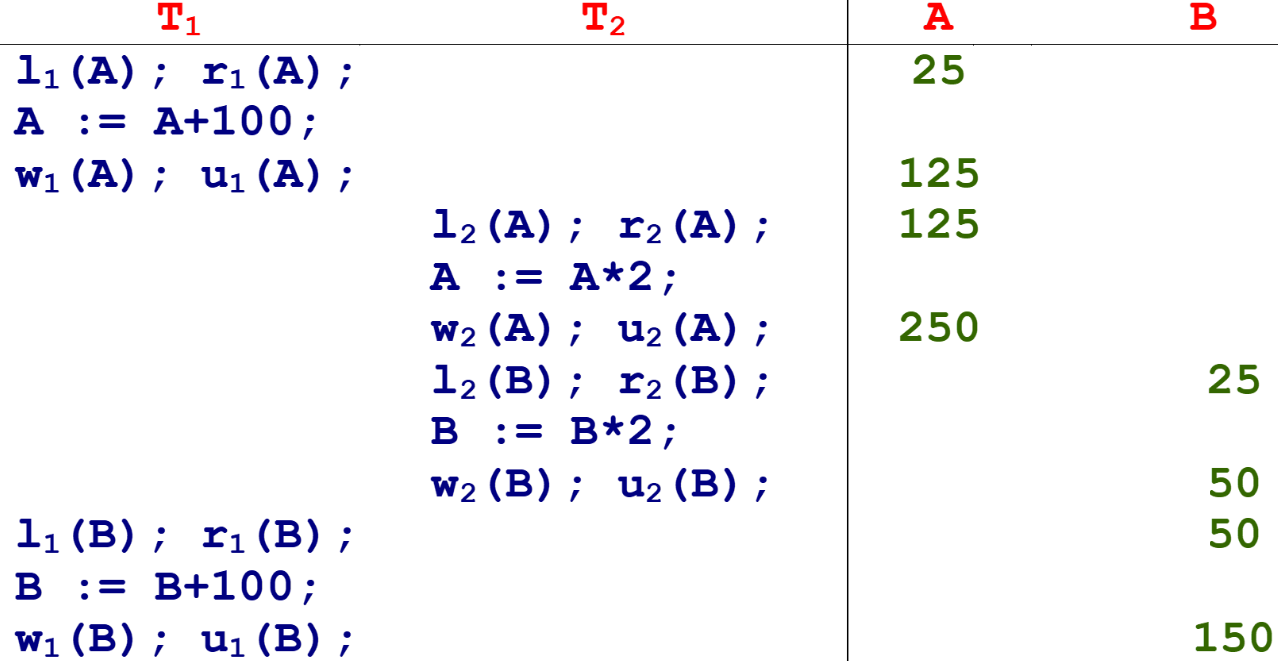
\includegraphics[height=6cm]{03.png}
		\end{figure}
		
		\item Megjegyzés:
		\begin{compactitem}
			\item Kibővítjük a jelöléseinket a zárolás és a feloldás műveletekkel:
			\begin{compactitem}
				\item l$ _{i} $(X): a T$ _{i} $ tranzakció az X adatbáziselemre zárolást kér (lock).
				\item u$ _{i} $(X): a T$ _{i} $ tranzakció az X adatbáziselem zárolását feloldja (unlock).
			\end{compactitem}
		\item Konzisztencia: Ha egy T$ _{i} $ tranzakcióban van egy r$ _{i} $(X) vagy egy w$ _{i} $(X) művelet, akkor van korábban egy l$ _{i} $(X) művelet, és van később egy u$ _{i} $(X) művelet, de a zárolás és az írás/olvasás között nincs u$ _{i} $(X).\\
		T$ _{i} $:  … l$ _{i} $(X) … r/w$ _{i} $(X) … u$ _{i} $(X) ...
		\end{compactitem}
	\end{compactitem}

213. Mit hívunk kétfázisú zárolásnak és szemléltessük rajzban is? (2 pont)
	\begin{compactitem}
		\item 
	\end{compactitem}
	
		
\end{document}